\chapter{Marco teórico y conceptual}
\label{cap:marco}

Este capítulo reúne los conceptos y los métodos en que se apoya el trabajo.

\section{Conceptos básicos}
\label{sec:conceptos}

\subsection{Imagen digital}

Una imagen digital en escala de grises, es decir, sin color, es una cuadrícula de $H$ filas y $W$
columnas de puntos llamados píxeles. Cada píxel guarda un número entero, su nivel de gris, que indica
cuán claro se ve ese punto \parencite{gonzalez2018}. En las imágenes de este trabajo, ese nivel va de 0,
el negro, a 255, el blanco. La fusión y las seis métricas que se usan aquí operan sobre la intensidad
normalizada, que lleva esos niveles al intervalo de cero a uno:
\begin{equation} f(x,y) = \frac{g(x,y)}{255}. \label{eq:intensidad} \end{equation}
En ella, $g(x,y)$ es el nivel de gris del píxel de la columna $x$ y la fila $y$, y $f(x,y)$ es su
intensidad normalizada. En adelante, la letra $f$ designa cualquier imagen normalizada.

\subsection{Imágenes visible e infrarroja}

La imagen visible (VIS) es la que toma una cámara común. Registra la luz que reflejan los objetos,
dentro de la franja que percibe el ojo humano. Por eso muestra bien la textura, los bordes y los
carteles, pero pierde calidad con poca luz o con mal tiempo. La imagen infrarroja térmica (IR) registra
en cambio el calor que emite cada cuerpo según su temperatura. Distingue a una persona o a un motor a
oscuras, aunque suele ofrecer menos detalle fino y poca textura \parencite{ma2019, bajacfigueredo2024}.
Aquí, la imagen visible en color se pasa a escala de grises antes de fusionarla.

Un par visible-infrarrojo está formado por dos imágenes de la misma escena, una de cada cámara, tomadas
al mismo tiempo. Para fusionarlas, las dos imágenes deben estar registradas, es decir, alineadas de modo
que un mismo píxel corresponda al mismo punto de la escena \parencite{gonzalez2018}. El registro corrige
las diferencias de posición, giro y tamaño que aparecen porque las cámaras no miran desde el mismo lugar.
Si el registro falla, el detalle de una imagen queda desplazado respecto del de la otra, y un borde puede
aparecer dos veces. Este trabajo no registra imágenes: usa conjuntos públicos cuyos pares ya vienen
registrados por sus autores.

\subsection{Niveles de fusión}

Las imágenes que se combinan se llaman fuentes. Según qué se combina, la fusión se clasifica en tres
niveles: de píxel, de características y de decisiones \parencite{singh2023}. El nivel de características
combina rasgos ya extraídos de cada fuente, como los bordes. El de decisiones combina los resultados de
sistemas que analizan cada fuente por separado, como dos detectores de objetos. El nivel de píxel
combina las fuentes punto por punto, sobre sus intensidades o sobre una versión transformada
\parencite{li2017}. Todos los métodos de este trabajo son de este último nivel. Su resultado
es una imagen del mismo tamaño que las fuentes:
\begin{equation} F = \Phi\left(I_{\mathrm{VIS}},\, I_{\mathrm{IR}}\right). \label{eq:fusion-pixel} \end{equation}
En ella, $I_{\mathrm{VIS}}$ e $I_{\mathrm{IR}}$ son las fuentes visible e infrarroja normalizadas, $\Phi$
es el método de fusión y $F$ es la imagen fusionada. Aquí $F$ también toma valores entre cero y uno,
porque todos los métodos recortan su resultado a ese intervalo.

\subsection{Evaluación sin imagen de referencia}

En la fusión de imágenes no siempre existe una imagen de referencia, es decir, una imagen fusionada
correcta con la cual comparar el resultado \parencite{singh2023}. En la fusión visible-infrarroja no existe,
porque ninguna cámara puede tomar la imagen ideal que reúna lo mejor de las dos. Por eso la calidad se
estima con métricas sin referencia, indicadores numéricos que no necesitan esa imagen. Unas se calculan
sobre la imagen fusionada sola y miden cuánta información, contraste o nitidez contiene. Otras la
comparan con cada fuente y miden cuánto conserva de la visible y de la infrarroja. Como cada métrica
premia una propiedad distinta, dos métricas pueden ordenar de manera diferente a los mismos métodos. La
Sección~\ref{sec:metricas} presenta las que se usan aquí.

\section{Fusión de imágenes visibles e infrarrojas}
\label{sec:fusion}

Cada cámara capta una parte de la escena y pierde otra. La fusión visible-infrarroja reúne en una sola
imagen la textura de la visible y el calor de la infrarroja \parencite{ma2019}. Sus usos van de la
vigilancia a la detección y el seguimiento de objetos \parencite{li2017, zhang2023}. Las revisiones del
área agrupan los métodos de fusión en varias familias \parencite{li2017, ma2019, singh2023}.

\subsection{Familias de métodos}

Una de las familias más difundidas es la multiescala \parencite{li2017}. Sus métodos descomponen cada
imagen en una base, con el brillo general, y en capas de detalle de distintos tamaños. Luego combinan
cada capa con su propia regla y reconstruyen el resultado. Son de este tipo las pirámides, que
representan la imagen a resoluciones cada vez menores, y las transformadas \textit{wavelet}, que la
analizan con ondas breves. También lo son los cinco métodos multiescala con que se compara la propuesta,
descritos en la Sección~\ref{sec:comparativos}.

Otra familia usa representaciones dispersas: cada bloque pequeño de la imagen se escribe como la suma de
pocos patrones tomados de un repertorio llamado diccionario, cada uno con su peso. En la fusión
visible-infrarroja, \textcite{wang2014} aplican esa idea sin admitir pesos negativos.

Una tercera familia usa redes neuronales, modelos que aprenden a fusionar a partir de ejemplos
\parencite{zhang2023}. FusionGAN, por ejemplo, enfrenta dos redes: una produce la imagen fusionada y la
otra la juzga. Así, la regla de fusión se aprende de los ejemplos en lugar de diseñarse a mano
\parencite{ma2019b}. Por eso, estos métodos necesitan entrenarse antes de usarse. Los métodos
morfológicos, en cambio, siguen pasos explícitos: extraen el detalle comparando la imagen con una figura
pequeña de forma conocida \parencite{serra1982}. La propuesta de este trabajo pertenece a este grupo.
Sus herramientas y su uso en la fusión se presentan en la Sección~\ref{sec:morfologia}.

\subsection{Métodos multiescala comparativos}
\label{sec:comparativos}

La propuesta se compara con cinco métodos multiescala y con el Top-Hat clásico, que se presenta en la
Sección~\ref{sec:fusion-tophat}. Los cinco multiescala separan cada imagen en capas de distinto detalle,
las combinan y reconstruyen la imagen fusionada. En los cinco métodos, el resultado se recorta al
intervalo de cero a uno.

\subsubsection{Pirámide de Laplace}

La pirámide de Laplace \parencite{burt1983} se propuso como método de codificación compacta de
imágenes. Usa copias $G_\ell$ cada vez más suaves y reducidas a la mitad, desde $G_0$, que es la imagen.
Cada capa $L_\ell$ guarda lo que se pierde al reducir. Con $K$ capas,
\begin{equation} L_\ell = G_\ell - \operatorname{amp}(G_{\ell+1}), \quad \ell = 0, 1, \ldots, K-2, \qquad L_{K-1} = G_{K-1}. \label{eq:laplace} \end{equation}
Aquí $\operatorname{amp}(\cdot)$ amplía una copia al doble y la suaviza. La capa fusionada $L^F_\ell$,
incluida la más gruesa, toma en cada píxel el valor de la fuente de mayor actividad local. Esa actividad
es el valor absoluto de la capa, suavizado en una ventana cuadrada que pesa más el centro. Para
reconstruir, se amplía $L^F_{K-1}$, se le suma $L^F_{K-2}$ y se repite el paso hasta $L^F_0$.

\subsubsection{Pirámide de razón}

La pirámide de razón de \textcite{toet1989}, pensada para la fusión, divide en lugar de restar. Con $K$
niveles usa $K+1$ de esas copias, de $G_0$ a $G_K$:
\begin{equation} R_\ell = \frac{G_\ell + \eta}{\operatorname{amp}(G_{\ell+1}) + \eta}, \qquad \ell = 0, 1, \ldots, K-1. \label{eq:razon} \end{equation}
La constante $\eta$ evita dividir por cero. Una razón igual a uno indica que no hay contraste local. Si
es mayor que uno, el punto es más claro que su entorno, y si es menor, más oscuro. En cada píxel, la
razón fusionada $R^F_\ell$ es la más alejada de uno, la de mayor contraste. La copia fusionada más
gruesa, $G^F_K$, es el promedio de las dos $G_K$. Desde ella se reconstruye por multiplicación:
\begin{equation} G^F_\ell = R^F_\ell \left[ \operatorname{amp}(G^F_{\ell+1}) + \eta \right], \qquad \ell = K-1, \ldots, 1, 0. \label{eq:razon-reconstruccion} \end{equation}
La imagen fusionada es $G^F_0$.

\subsubsection{Transformada \textit{wavelet} discreta}

La transformada \textit{wavelet} discreta (DWT, del inglés \textit{Discrete Wavelet Transform}) mide los
cambios de la imagen con una \textit{wavelet}, una onda breve usada como patrón. En cada nivel separa la
imagen en una aproximación suavizada, de alrededor de la mitad de ancho y alto, y tres detalles:
horizontal, vertical y diagonal \parencite{gonzalez2018}. El proceso se repite sobre la aproximación, y
cada valor obtenido es un coeficiente. El trabajo de \textcite{li1995} la aplica a la fusión de imágenes
de distintos sensores. La primera de las dos DWT comparadas, llamada DWT (Haar), usa la base de Haar. Esa base es la
onda más simple: suma y resta píxeles vecinos por pares \parencite{gonzalez2018}. La aproximación $A$ se
promedia. Cada coeficiente de detalle $D$ se toma de la fuente en que es mayor en valor absoluto:
\begin{equation} A^F=\tfrac{1}{2}\bigl(A^{\mathrm{VIS}}+A^{\mathrm{IR}}\bigr), \qquad D^F=\begin{cases} D^{\mathrm{VIS}} & \text{si } |D^{\mathrm{VIS}}|\geq|D^{\mathrm{IR}}|,\\ D^{\mathrm{IR}} & \text{en otro caso}. \end{cases} \label{eq:regla-wavelet} \end{equation}

\subsubsection{Transformada \textit{wavelet} compleja de doble árbol}

Según \textcite{kingsbury2001}, la DWT tiene dos límites: sus coeficientes cambian mucho si la imagen se
desplaza un píxel, y solo distingue tres direcciones. La transformada \textit{wavelet} compleja de doble
árbol (DTCWT, del inglés \textit{Dual-Tree Complex Wavelet Transform}) busca un análisis casi invariante
al desplazamiento, es decir, estable ante esos cambios. Usa dos cadenas de filtros en paralelo, llamadas
árboles; un filtro es una operación que deja pasar solo ciertos detalles. Las salidas de los
árboles forman coeficientes complejos, números con una parte real y otra imaginaria. El módulo de cada coeficiente, que
reúne las dos partes en un solo valor, varía poco ante desplazamientos pequeños. Cada nivel ofrece,
además, seis orientaciones. Para fusionar se aplica la regla de la Ecuación~\eqref{eq:regla-wavelet},
con el módulo en lugar del valor absoluto.

\subsubsection{Transformada \textit{wavelet} discreta con la base de Daubechies}

El quinto método multiescala es una segunda DWT, con la regla de la
Ecuación~\eqref{eq:regla-wavelet} y la base de Daubechies de orden cuatro \parencite{daubechies1988}. Esa base tiene filtros más
largos y una onda más suave que la de Haar. Como sigue siendo una DWT, distingue las mismas tres
direcciones. En adelante se la llama DWT (db4), para distinguirla de la DWT (Haar).

\section{Morfología matemática y transformada Top-Hat}
\label{sec:morfologia}

La morfología matemática analiza la forma de las estructuras de una imagen \parencite{serra1982}. Para
eso la compara con una figura pequeña de forma conocida, llamada elemento estructurante, que se desplaza
por todos los píxeles. En escala de grises, cada nivel de gris se lee como una altura, y la imagen se ve
como un relieve de montes claros y valles oscuros. El elemento estructurante $b$ es el conjunto de
desplazamientos $(j,k)$ de sus píxeles respecto de su centro, e incluye al centro mismo. El
desplazamiento $j$ se mide en columnas y $k$ en filas, como $x$ e $y$ en la imagen. La forma y el tamaño
del elemento deciden qué detalles se conservan.

\subsection{Operaciones básicas}

Las operaciones morfológicas parten de dos básicas, la erosión y la dilatación
\parencite{soille2003, gonzalez2018}. La erosión, $\varepsilon$, toma en cada píxel el menor nivel de
gris bajo el elemento centrado en él, y la dilatación, $\delta$, el mayor:
\begin{equation} \varepsilon(f,b)(x,y) = \min_{(j,k)\in b} f(x+j,\, y+k), \qquad \delta(f,b)(x,y) = \max_{(j,k)\in b} f(x+j,\, y+k). \label{eq:erosion-dilatacion} \end{equation}
Los vecinos que caen fuera de la imagen se ignoran. El elemento es plano: solo indica qué vecinos se
comparan. La erosión angosta los montes y borra los más estrechos que el elemento, y la dilatación hace
lo mismo con los valles. Algunos textos, como el de \textcite{gonzalez2018}, giran el elemento media
vuelta en la dilatación. Con elementos simétricos respecto de su centro, como los de este trabajo, ese
giro no cambia el resultado.

La apertura, $\gamma$, es una erosión seguida de una dilatación con el mismo elemento. El cierre,
$\varphi$, es una dilatación seguida de una erosión:
\begin{equation} \gamma(f,b) = \delta\bigl(\varepsilon(f,b),\, b\bigr), \qquad \varphi(f,b) = \varepsilon\bigl(\delta(f,b),\, b\bigr). \label{eq:apertura-cierre} \end{equation}
La apertura rebaja los montes en los que el elemento no cabe hasta la altura en que sí cabe, y deja casi
intacto el resto. El cierre rellena, del mismo modo, los valles en los que el elemento no cabe. Por eso
la apertura nunca supera a la imagen y el cierre nunca queda por debajo de ella \parencite{soille2003}.
La Figura~\ref{fig:morfologia} muestra el efecto de estas cuatro operaciones sobre una señal de una
dimensión, como los niveles de gris a lo largo de una fila. Su último panel anticipa la transformada
Top-Hat, que se define a continuación.

\begin{figure}[htbp]
\centering
\caption{Operaciones morfológicas básicas y transformada Top-Hat sobre una señal de una dimensión}
\label{fig:morfologia}
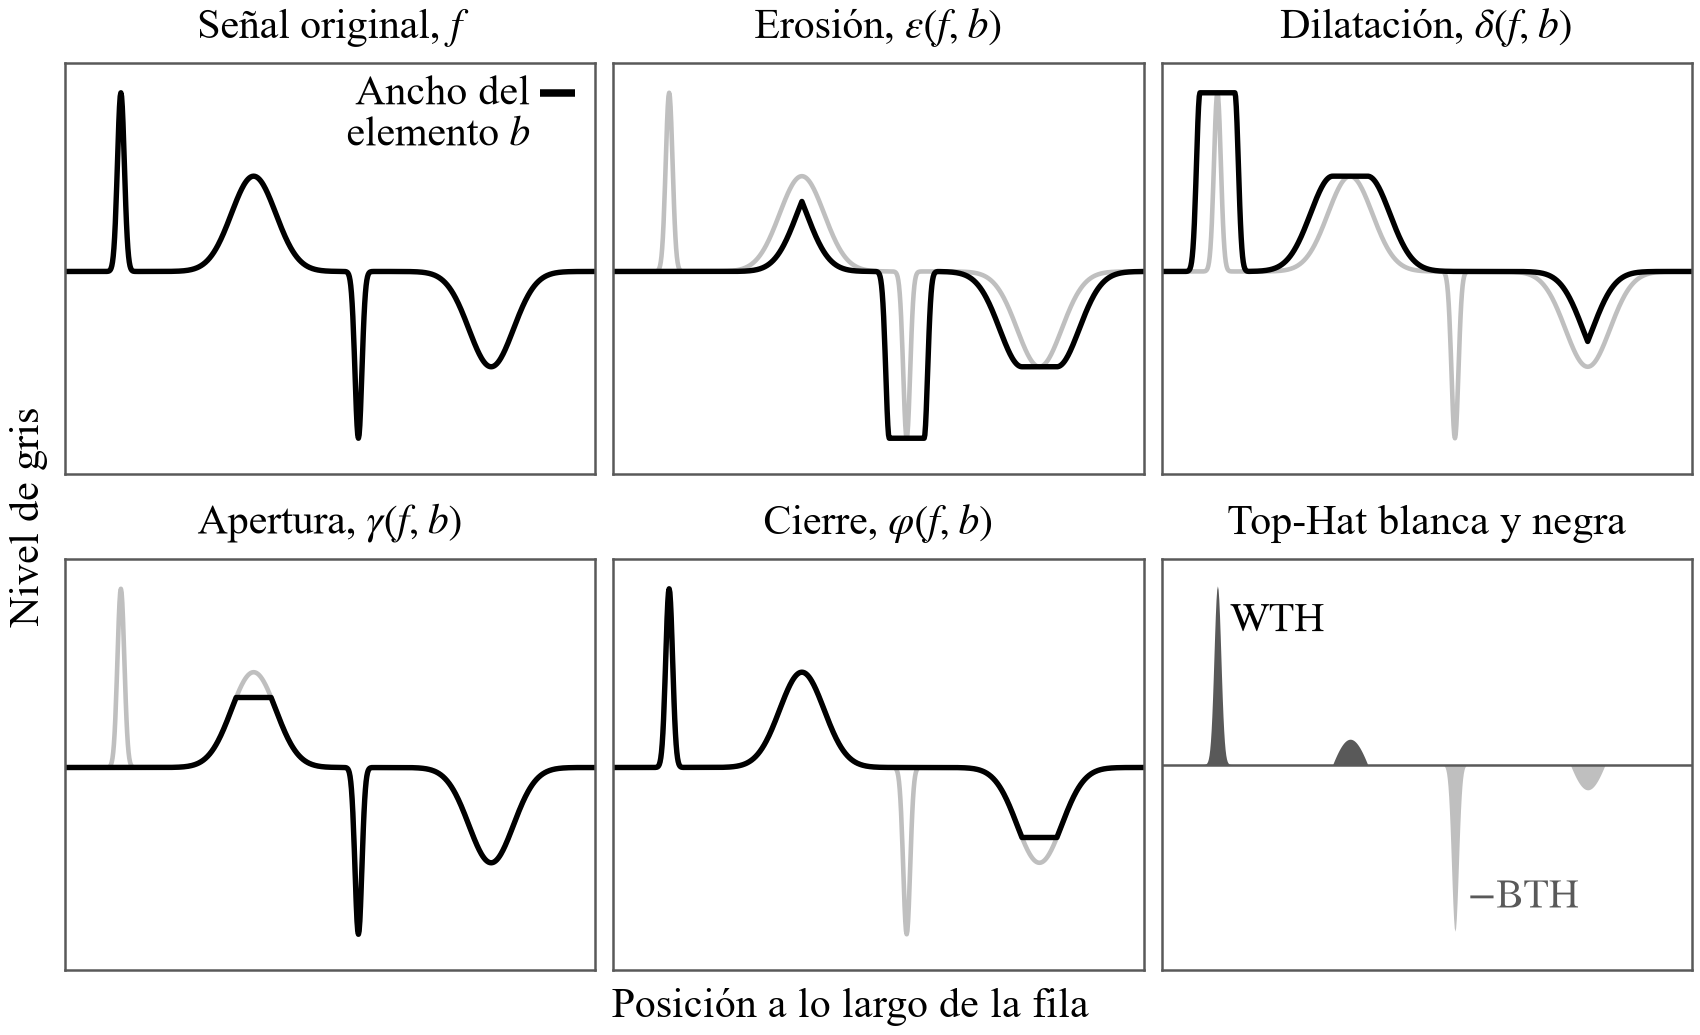
\includegraphics[width=0.9\textwidth]{figuras/fig_morfologia_tophat}
\nota{Elaboración propia. La barra del primer panel marca el ancho del elemento estructurante $b$. En
los cuatro paneles siguientes se repite en gris la señal original $f$. En el último, la Top-Hat blanca
se dibuja hacia arriba y la negra, con el signo cambiado, hacia abajo. Los montes y valles más
estrechos que $b$ pasan enteros a la Top-Hat; de los más anchos, solo pasa la parte más estrecha que $b$.}
\end{figure}

\subsection{Transformada Top-Hat}

La transformada Top-Hat mide cuánto cambia la imagen al aplicarle la apertura o el cierre. La Top-Hat
blanca (WTH, del inglés \textit{White Top-Hat}) es la imagen menos su apertura. La negra (BTH, del inglés
\textit{Black Top-Hat}) es el cierre menos la imagen \parencite{soille2003, gonzalez2018}:
\begin{equation} \mathrm{WTH}(f,b) = f - \gamma(f,b), \qquad \mathrm{BTH}(f,b) = \varphi(f,b) - f. \label{eq:wth-bth} \end{equation}
La blanca conserva los detalles claros más estrechos que el elemento, y la negra, los oscuros. Las dos
son mayores o iguales que cero, y casi nulas en las zonas planas o de variación suave. Así separan el
detalle fino, que queda en las dos Top-Hat, del fondo, que queda en la apertura y en el cierre.

\subsection{Tamaño y forma del elemento estructurante}

El tamaño del elemento fija la frontera entre el detalle y el fondo \parencite{soille2003, gonzalez2018}.
De cada monte o valle, la Top-Hat recoge la parte más estrecha que el elemento, y el resto queda en el
fondo. Con un elemento pequeño, la Top-Hat recoge solo la textura fina, las líneas delgadas y el ruido.
Con uno grande puede recoger además objetos enteros, como una persona o un vehículo que se destacan de su
entorno. En este trabajo el tamaño se expresa con un radio $r$, en píxeles, y cada elemento se extiende
unos $r$ píxeles a cada lado de su centro.

La forma del elemento decide en qué direcciones se mide ese ancho \parencite{serra1982, soille2003}. Un
disco mide lo mismo en todas las direcciones y no distingue la orientación de los detalles. Un segmento
de recta, en cambio, mira en una sola dirección. La apertura con un segmento conserva las estructuras
claras que se extienden en esa dirección al menos tanto como el segmento, y rebaja las demás. Por eso el
segmento no extrae las estructuras alineadas con él: como cabe en ellas, estas sobreviven a la apertura y
la Top-Hat vale cero allí. Extrae, en cambio, los detalles más angostos que su largo en esa dirección.
Así, un objeto alargado queda en el fondo con un segmento paralelo y pasa a la Top-Hat con uno
perpendicular más largo que su ancho.

\subsection{Realce de contraste}

La Top-Hat sirve también para realzar el contraste, es decir, para que un detalle se distinga mejor de
su entorno. Su forma más simple suma a la imagen su Top-Hat blanca y le resta la negra
\parencite{bai2012}:
\begin{equation} f_{\mathrm{R}} = f + \mathrm{WTH}(f,b) - \mathrm{BTH}(f,b). \label{eq:realce} \end{equation}
Aquí $f_{\mathrm{R}}$ es la imagen realzada. Los detalles claros se aclaran, los oscuros se oscurecen y
el fondo casi no cambia. Los trabajos de \textcite{mukhopadhyay2000} y \textcite{bai2012} llevan esta
idea a varias escalas, con elementos de tamaños crecientes. Algunos métodos morfológicos de fusión la
aplican a dos imágenes a la vez \parencite{bai2013, roman2020}, y así lo hace también el algoritmo
propuesto.

\subsection{Fusión basada en la transformada Top-Hat}
\label{sec:fusion-tophat}

En su versión más simple, la fusión basada en la transformada Top-Hat separa en cada fuente el detalle
del fondo y agrega el detalle de ambas a una imagen base común \parencite{roman2020,
ortegarodriguez2025}. La regla siguiente es común al Top-Hat clásico y a la propuesta. Retoma la de
\textcite{ortegarodriguez2025}, incluido el peso que regula cuánto detalle se agrega, y recorta el
resultado de forma explícita al intervalo de cero a uno. Sean $\mathrm{WTH}_{\mathrm{VIS}}$ y
$\mathrm{BTH}_{\mathrm{VIS}}$ las transformadas Top-Hat blanca y negra de la visible, y
$\mathrm{WTH}_{\mathrm{IR}}$ y $\mathrm{BTH}_{\mathrm{IR}}$ las de la infrarroja. La imagen fusionada es
\begin{equation} \begin{aligned} F = \operatorname{recorte}\Bigl( & \tfrac{1}{2}\bigl(I_{\mathrm{VIS}} + I_{\mathrm{IR}}\bigr)
 + m \max\bigl(\mathrm{WTH}_{\mathrm{VIS}},\, \mathrm{WTH}_{\mathrm{IR}}\bigr) \\
 & - m \max\bigl(\mathrm{BTH}_{\mathrm{VIS}},\, \mathrm{BTH}_{\mathrm{IR}}\bigr) \Bigr). \end{aligned} \label{eq:regla-tophat} \end{equation}
Aquí $m$ es un peso no negativo, y el máximo se toma píxel a píxel. La función
$\operatorname{recorte}(z) = \min\{1, \max\{0, z\}\}$ lleva a cero los valores negativos y a uno los
mayores que uno.

La regla parte del promedio de las dos fuentes, que hace de imagen base. En cada píxel toma el mayor
detalle claro y el mayor detalle oscuro de las dos fuentes, así que un detalle se conserva si al menos
una de las cámaras lo capta. El claro se suma a la base y el oscuro se resta. Como las transformadas
Top-Hat nunca son negativas, la suma aclara los detalles claros y la resta oscurece los oscuros. Así crece
el contraste local, la diferencia de brillo entre un detalle y su entorno. Con $m = 0$ la fusión es el
promedio simple, y cuanto mayor es $m$, más detalle se agrega. Un peso alto puede sacar más píxeles del
intervalo de cero a uno, que el recorte deja en negro o en blanco. El Top-Hat clásico sigue la fusión
con Top-Hat de \textcite{bajacfigueredo2024} y aplica esta regla con un único disco como elemento
estructurante.

\section{Métricas de evaluación sin referencia}
\label{sec:metricas}

La calidad de una fusión visible-infrarroja se estima con métricas que no necesitan una imagen fusionada
ideal \parencite{ma2019, singh2023}. Para \textcite{singh2023}, sin referencia son solo las que usan la
fusión sola; las que la comparan con las fuentes son de referencia parcial. Aquí se usan seis, en
dos grupos de tres. Las del primer grupo miden la actividad: cuánta información, cuánto contraste y
cuánta nitidez de bordes tiene la fusión por sí misma. Las del segundo miden la fidelidad, es decir,
cuánto se parece la fusión a cada fuente. En las seis, un valor mayor se considera mejor. En lo que
sigue, $F$ es la imagen fusionada, de $H$ filas y $W$ columnas, y $X$ designa una fuente, sea
$I_{\mathrm{VIS}}$ o $I_{\mathrm{IR}}$.

\subsection{Métricas de actividad}

Las tres métricas de actividad son la entropía (EN, del inglés \textit{Entropy}), la desviación estándar
(SD, del inglés \textit{Standard Deviation}) y el gradiente medio (MG, del inglés \textit{Mean Gradient}).

La entropía mide cuán repartidos están los píxeles entre los niveles de gris
\parencite{singh2023, ortegarodriguez2025}. Para calcularla, el
intervalo de cero a uno se divide en 256 tramos iguales, y $p_a$ es la proporción de píxeles de $F$ que
caen en el tramo $a$. Ese reparto se llama histograma. La entropía es
\begin{equation} \mathrm{EN}(F) = -\sum_{a=0}^{255} p_a \log_2 p_a. \label{eq:met-en} \end{equation}
Los tramos vacíos no aportan. Se mide en bits, la unidad de información, y alcanza su máximo, 8~bits,
cuando todos los tramos tienen la misma proporción.

La desviación estándar mide el contraste general, es decir, cuánto se alejan en promedio las
intensidades de su valor medio $\mu_F$ \parencite{singh2023, ortegarodriguez2025}. Una imagen de tono
parejo tiene una desviación baja, y una con zonas muy claras junto a zonas muy oscuras la tiene alta. Se
calcula como
\begin{equation} \mathrm{SD}(F) = \sqrt{\frac{1}{HW}\sum_{x=1}^{W}\sum_{y=1}^{H}\bigl(F(x,y)-\mu_F\bigr)^2}, \qquad \mu_F = \frac{1}{HW}\sum_{x=1}^{W}\sum_{y=1}^{H}F(x,y). \label{eq:met-sd} \end{equation}
Aquí $F(x,y)$ es la intensidad del píxel de la columna $x$ y la fila $y$. La suma de cuadrados se
divide por el número total de píxeles, $HW$. Como las intensidades van de cero a uno, SD no puede
superar 0.5. Su cuadrado se llama varianza.

El gradiente medio mide la nitidez de los bordes \parencite{singh2023}. El gradiente indica cuánto cambia
la intensidad de un píxel a sus vecinos, y crece donde la imagen salta de claro a oscuro. En el interior
de la imagen se calcula con diferencias centrales, entre el vecino anterior y el siguiente:
\begin{equation} G_x(x,y) = \frac{F(x+1,y)-F(x-1,y)}{2}, \qquad G_y(x,y) = \frac{F(x,y+1)-F(x,y-1)}{2}. \label{eq:met-gradiente} \end{equation}
Aquí $G_x$ es el cambio horizontal y $G_y$ el vertical. En las filas y columnas extremas, donde falta un
vecino, se usa la diferencia con el único disponible, sin dividir por dos. Así,
\begin{equation} \mathrm{MG}(F) = \frac{1}{HW}\sum_{x=1}^{W}\sum_{y=1}^{H}\sqrt{G_x(x,y)^2+G_y(x,y)^2}. \label{eq:met-mg} \end{equation}
El valor depende de la fórmula de las diferencias, así que solo se comparan valores calculados de la
misma manera.

\subsection{Métricas de fidelidad}

Las tres métricas de fidelidad son la información mutua (MI, del inglés \textit{Mutual Information}), la
similitud estructural (SSIM, del inglés \textit{Structural Similarity}) y la relación señal-ruido de pico
(PSNR, del inglés \textit{Peak Signal-to-Noise Ratio}).

La información mutua mide cuánto baja la incertidumbre sobre el nivel de gris de un píxel en una fuente
$X$ al conocer su nivel en $F$ \parencite{qu2002}. Para calcularla, cada intensidad se multiplica por 63
y se trunca al entero inferior, lo que deja 64 niveles. Con ellos se arma el histograma conjunto, donde
$p_{FX}(a,c)$ es la proporción de píxeles con nivel $a$ en $F$ y nivel $c$ en $X$. Así,
\begin{equation} \mathrm{MI}(F,X) = \sum_{a=0}^{63}\sum_{c=0}^{63} p_{FX}(a,c)\,\log_2\frac{p_{FX}(a,c)}{p_F(a)\,p_X(c)}. \label{eq:met-mi} \end{equation}
Aquí $p_F(a)$ y $p_X(c)$ son las proporciones en cada imagen sola, y las casillas vacías no aportan. La
métrica del trabajo promedia las dos fuentes en cada par de imágenes:
\begin{equation} \mathrm{MI} = \tfrac{1}{2}\bigl[\mathrm{MI}(F,I_{\mathrm{VIS}})+\mathrm{MI}(F,I_{\mathrm{IR}})\bigr]. \label{eq:met-mi-promedio} \end{equation}
Si se sumaran los dos términos, el valor se duplicaría sin cambiar el orden de los métodos.

El índice de similitud estructural compara dos imágenes por zonas pequeñas, o ventanas
\parencite{wang2004}. En cada ventana $w$ compara el brillo medio, el contraste y el patrón de variación
de $X$ y de $F$:
\begin{equation} \mathrm{SSIM}_w(X,F) = \frac{(2\mu_X\mu_F + C_1)(2\sigma_{XF} + C_2)}{(\mu_X^2+\mu_F^2+C_1)(\sigma_X^2+\sigma_F^2+C_2)}. \label{eq:met-ssim} \end{equation}
Aquí $\mu_X$ y $\mu_F$ son las medias en la ventana, $\sigma_X^2$ y $\sigma_F^2$ las varianzas, y
$\sigma_{XF}$ la covarianza, que mide cuánto varían juntas. Las constantes $C_1=(0.01)^2$ y
$C_2=(0.03)^2$ evitan dividir por cero. En este trabajo la ventana mide $7 \times 7$ píxeles, todos
con el mismo peso, y las varianzas y la covarianza se dividen por 48. La versión original usa una ventana mayor que
pesa más el centro \parencite{wang2004}. El índice promedia $\mathrm{SSIM}_w$ sobre las ventanas que
caben enteras, y la métrica final promedia las dos fuentes:
\begin{equation} \mathrm{SSIM} = \tfrac{1}{2}\bigl[\mathrm{SSIM}(I_{\mathrm{VIS}},F)+\mathrm{SSIM}(I_{\mathrm{IR}},F)\bigr]. \label{eq:met-ssim-promedio} \end{equation}

La relación señal-ruido de pico expresa el error numérico entre dos imágenes en escala logarítmica, que
reúne en un rango corto valores muy distintos \parencite{singh2023}. Se apoya en el error cuadrático
medio (MSE, del inglés \textit{Mean Squared Error}), el promedio de los cuadrados de las diferencias
píxel a píxel. Siguiendo a \textcite{ortegarodriguez2025}, primero se promedian los errores frente a
las dos fuentes y después se toma el logaritmo. Así,
\begin{equation} \begin{aligned} \mathrm{MSE}(F,X) &= \frac{1}{HW}\sum_{x=1}^{W}\sum_{y=1}^{H}\bigl(F(x,y)-X(x,y)\bigr)^2,\\
 \mathrm{PSNR} &= 10\log_{10}\frac{1}{\tfrac{1}{2}\bigl[\mathrm{MSE}(F,I_{\mathrm{VIS}})+\mathrm{MSE}(F,I_{\mathrm{IR}})\bigr]}. \end{aligned} \label{eq:met-psnr} \end{equation}
El 1 del numerador es el cuadrado de la mayor intensidad posible. La PSNR se mide en decibelios, la
unidad de esa escala, y un valor alto indica que la fusión se aparta poco de sus fuentes. En la escala de
0 a 255 el valor no cambia, porque el numerador y el error crecen en la misma proporción. Promediar los
errores no equivale a promediar las dos PSNR.

\subsection{Selección de las seis métricas}

Las seis resultan de depurar con dos criterios una batería inicial de nueve métricas. Esa batería
incluye las cinco que usan \textcite{ortegarodriguez2025}. El primer criterio es no repetir información. La
eficiencia de fusión (FE, del inglés \textit{Fusion Efficiency}) divide la EN de la fusión por la EN
media de las fuentes. Como ese divisor es fijo en cada par, FE ordena los métodos igual que EN. La
frecuencia espacial (SF, del inglés \textit{Spatial Frequency}) mide el cambio entre píxeles vecinos
\parencite{eskicioglu1995}, casi lo mismo que MG. La batería contaba aparte la MI con cada fuente, lo
que duplicaba su peso. Sin esas tres repeticiones quedan las seis. El segundo criterio es el equilibrio.
La actividad sube también con el ruido, y la fidelidad, con solo copiar las fuentes; por eso los dos
grupos tienen tres métricas cada uno.

\subsection{Métricas complementarias}

Otras ocho métricas se calculan solo como comprobación, y el Capítulo~\ref{cap:resultados} las usa con
ese fin. El índice de información de bordes (Qabf) mide cuánta información de bordes pasa de las fuentes
a la fusión \parencite{xydeas2000}. La medida de ruido y artefactos de fusión (Nabf) se propuso después en
ese marco \parencite{petrovic2005}. Pondera los píxeles donde la fusión tiene bordes más fuertes que las
dos fuentes, y es la única en que un valor menor es mejor. Aquí se usa la ponderación modificada de
\textcite{kumar2013}. La suma de las correlaciones de las diferencias (SCD, del inglés \textit{Sum of the
Correlations of Differences}) suma, para cada fuente, su correlación con la diferencia entre la imagen
fusionada y la otra fuente \parencite{aslantas2015}. La fidelidad de la información visual (VIF, del
inglés \textit{Visual Information Fidelity}) mide cuánta información visual de un original conserva otra
imagen \parencite{sheikh2006}; aquí, el original es cada fuente. La información mutua de
características (FMI, del inglés \textit{Feature Mutual Information}) aplica la información mutua a los
gradientes \parencite{haghighat2011}. Las tres variantes de \textcite{piella2003} calculan por
ventanas el índice de la Ecuación~\eqref{eq:met-ssim} sin $C_1$ ni $C_2$ y combinan esos valores con
distintos pesos. Son el índice ponderado por la varianza local (Q0), el ponderado por ventana (QW) y el
de bordes (QE). En el primero, el índice de cada fuente pesa en cada ventana según su varianza local. El
segundo da además más peso a las ventanas de mayor varianza, y el tercero multiplica QW por el mismo
índice calculado sobre los bordes de las imágenes. En esa obra el primero se llama Q; aquí figura como
Q0, aunque sus autores reservan ese nombre para el índice sin ponderar. Las ocho comparan la fusión con
sus fuentes, y sumarlas inclinaría el equilibrio hacia la fidelidad.

\section{Pruebas estadísticas}
\label{sec:pruebas}

Para comparar la calidad de los métodos se usan pruebas no paramétricas, que no suponen una distribución
normal de los datos. La prueba de Friedman \parencite{friedman1937} trata cada par de imágenes como un bloque:
ordena los métodos dentro de cada par y pregunta si alguno tiende a quedar mejor o peor ubicado. La prueba de
Wilcoxon de rangos con signo \parencite{wilcoxon1945} compara dos métodos a partir de sus diferencias en
los mismos pares. Cada prueba da un valor de $p$: la probabilidad de ver una diferencia al menos tan
grande si los métodos fueran iguales. Como las comparaciones por pares son muchas, esos valores se
corrigen con el procedimiento de \textcite{holm1979}. Ese procedimiento los ordena de menor a mayor y los
compara con umbrales que empiezan muy estrictos y se aflojan paso a paso.

Cuando las observaciones de un mismo grupo no son independientes, como los cuadros de un mismo tramo de
video, el error estándar se calcula por grupos y no por observación \parencite{cameron2015}. Con pocos
grupos, ese error tiende a subestimar la variación, y el \textit{bootstrap} salvaje por grupos
estudentizado ofrece una prueba más confiable \parencite{cameron2008, webb2023}. Este repite el cálculo
miles de veces, con el aporte de cada grupo multiplicado por un peso al azar, y en cada repetición
divide la estimación por su propio error estándar. La correlación de rangos de Spearman
\parencite{spearman1904}, por último, mide cuánto coinciden dos ordenamientos de los mismos elementos.

\section{Optimización por enjambre de partículas}
\label{sec:pso}

La optimización por enjambre de partículas (PSO, del inglés \textit{Particle Swarm Optimization}) es un
método de búsqueda propuesto por \textcite{kennedy1995}. El método mueve un grupo de soluciones
posibles, llamadas partículas, dentro de una región de búsqueda. En la fusión de imágenes, \textcite{tao2010}
combinan la PSO con la DTCWT, y \textcite{malviya2014}, con la transformada \textit{wavelet}. Por su parte,
\textcite{ortegarodriguez2025} la aplican a los parámetros de la transformada Top-Hat en la fusión
visible-infrarroja.

La búsqueda avanza por iteraciones, es decir, por pasos sucesivos. En la iteración $t$, la partícula
$i$ ocupa la posición $\mathbf{x}_i^{t}$ y tiene la velocidad $\mathbf{v}_i^{t}$, que indica hacia
dónde y cuánto se desplaza. Al comenzar, las posiciones y las
velocidades se sortean al azar. Cada partícula recuerda la mejor posición que ha visitado,
$\mathbf{p}_i^{t}$, y conoce la mejor posición del grupo, $\mathbf{g}^{t}$. Para decidir cuál es mejor
se usa una función de aptitud, que asigna a cada posición un número, mayor cuanto mejor es la solución.
En cada iteración se evalúan las partículas y se actualizan esas mejores posiciones. Luego cada partícula
cambia su velocidad:
\begin{equation} \mathbf{v}_i^{t+1} = w_t\,\mathbf{v}_i^{t} + c_1\,\boldsymbol{\rho}_1 \odot \bigl(\mathbf{p}_i^{t} - \mathbf{x}_i^{t}\bigr) + c_2\,\boldsymbol{\rho}_2 \odot \bigl(\mathbf{g}^{t} - \mathbf{x}_i^{t}\bigr). \label{eq:pso-velocidad} \end{equation}
Con ella, la nueva posición es
\begin{equation} \mathbf{x}_i^{t+1} = \min\bigl(\max\bigl(\mathbf{x}_i^{t} + \mathbf{v}_i^{t+1},\, \mathbf{x}_{\min}\bigr),\, \mathbf{x}_{\max}\bigr). \label{eq:pso-posicion} \end{equation}

Los vectores $\boldsymbol{\rho}_1$ y $\boldsymbol{\rho}_2$ contienen números al azar entre cero y uno,
todos igual de probables. Se sortean de nuevo en cada iteración, para cada partícula y cada coordenada.
El símbolo $\odot$ indica el producto coordenada a coordenada. Los coeficientes $c_1$ y $c_2$ regulan
la atracción hacia la mejor posición propia y hacia la del grupo. En la
Ecuación~\eqref{eq:pso-posicion}, el mínimo y el máximo mantienen cada coordenada dentro de los límites
$\mathbf{x}_{\min}$ y $\mathbf{x}_{\max}$ de la región de búsqueda. El factor $w_t$, llamado inercia,
regula cuánto conserva cada partícula de su velocidad anterior. Ese factor no figura en la versión
original de \textcite{kennedy1995}; lo introducen \textcite{shi1998}.

Cuando la inercia decrece en línea recta a lo largo de las $T$ iteraciones, va de $w_{\max}$ en la
primera a $w_{\min}$ en la última. Su valor en la iteración $t$ es entonces
\begin{equation} w_t = w_{\max} - \left(w_{\max} - w_{\min}\right)\frac{t}{T-1}, \qquad t = 0, 1, \ldots, T-1. \label{eq:pso-inercia} \end{equation}
Con una inercia alta pesa más la velocidad anterior, y con una baja, la atracción hacia las mejores
posiciones halladas. Al terminar las iteraciones, la solución es la mejor posición del grupo.

\section{Detección de objetos}
\label{sec:marco-deteccion}

\subsection{Funcionamiento de un detector}

La detección automática de objetos consiste en encontrar y ubicar en una imagen los objetos de ciertas
clases, como personas o luces. El detector se entrena con imágenes en las que cada objeto está marcado
con una caja rectangular y su clase. Luego, ante una imagen nueva, devuelve predicciones: cajas con una
clase y un puntaje de confianza, que indica cuán seguro está el modelo. El detector YOLO
(del inglés \textit{You Only Look Once}, \enquote{solo se mira una vez}) propone las cajas y sus clases
en una sola pasada, al ritmo del video \parencite{redmon2016}. Su octava versión, YOLOv8, es de libre
distribución y ofrece cinco tamaños y pesos preentrenados, es decir, valores internos ya aprendidos con
otras imágenes \parencite{jocher2023}.

\subsection{Intersección sobre la unión, precisión y exhaustividad}

Para juzgar una predicción, su caja $B$ se compara con la caja marcada $A$. Se usa la intersección sobre
la unión (IoU, del inglés \textit{Intersection over Union}), con la que YOLO define también la
confianza de sus cajas \parencite{redmon2016}:
\begin{equation} \mathrm{IoU}(A,B)=\frac{\lvert A\cap B\rvert}{\lvert A\rvert+\lvert B\rvert-\lvert A\cap B\rvert}. \label{eq:iou} \end{equation}
Aquí $A\cap B$ es la zona común a las dos cajas, y $\lvert\cdot\rvert$ indica el área. La IoU vale uno si
las cajas coinciden y cero si no se superponen. Solo cuentan las predicciones cuyo puntaje de confianza
alcanza un umbral. Cada objeto marcado se une, como máximo, a una predicción de su misma clase: la de
mayor IoU entre las que siguen libres. En este trabajo, si esa IoU alcanza 0.5, el objeto cuenta como
encontrado. Ese umbral es el del desafío de reconocimiento visual de objetos PASCAL VOC (del inglés
\textit{Pattern Analysis, Statistical Modelling and Computational Learning Visual Object Classes}),
descrito por \textcite{everingham2010}. La predicción es entonces un verdadero positivo, $\mathit{VP}$,
y deja de estar libre.

Las predicciones que quedan libres son falsos positivos, $\mathit{FP}$, y los objetos sin pareja, falsos
negativos, $\mathit{FN}$. Con esos conteos se definen la precisión $P$ y la exhaustividad $R$:
\begin{equation} P=\frac{\mathit{VP}}{\mathit{VP}+\mathit{FP}},\qquad R=\frac{\mathit{VP}}{\mathit{VP}+\mathit{FN}}. \label{eq:precision-exhaustividad} \end{equation}
La primera mide qué parte de las predicciones es correcta; la segunda, qué parte de los objetos se
encuentra. Ambas dependen del umbral de confianza. Al bajarlo, $R$ crece o se mantiene, y $P$ suele
caer. La exhaustividad se llama también tasa de acierto. Calculada sobre un grupo elegido de objetos, es
la base de la medida de detección de este trabajo, descrita en la Sección~\ref{sec:protocolo-deteccion}.

\subsection{Precisión media}

La precisión media (AP, del inglés \textit{Average Precision}) resume la relación entre $P$ y $R$ en
todos los umbrales de confianza. Se calcula para cada clase por separado:
\begin{equation} \mathrm{AP}=\int_{0}^{1}\tilde{P}(R)\,dR. \label{eq:ap} \end{equation}
Aquí $\tilde{P}(R)$ es la mayor precisión lograda con una exhaustividad de $R$ o más. La integral se
aproxima con 101 valores de $R$ repartidos por igual entre cero y uno, como hace la biblioteca
Ultralytics \parencite{jocher2023}. La AP depende también del umbral
de IoU que decide los aciertos; con 0.5 se escribe AP50. La mAP50 es la media de la AP50 sobre las $C$
clases con objetos marcados:
\begin{equation} \mathrm{mAP50}=\frac{1}{C}\sum_{c=1}^{C}\mathrm{AP50}_c. \label{eq:map50} \end{equation}
Aquí $\mathrm{AP50}_c$ es la de la clase $c$.

\subsection{La detección como evaluación de la fusión}

La detección sirve también para evaluar una fusión. Esa evaluación exige cuidado, porque un detector
aprende la apariencia de sus imágenes de entrenamiento, como el contraste y la textura. Si se lo aplica
sin reentrenar a imágenes de otro aspecto, su acierto puede caer, como muestran \textcite{redmon2016}
con pinturas. Así, el resultado de la detección puede reflejar en parte ese cambio de aspecto, y no solo la utilidad
de la fusión.
Para comparar métodos en igualdad de condiciones, \textcite{liu2022} entrenan un detector con las
imágenes fusionadas de cada uno. Este trabajo sigue esa práctica, como detalla la
Sección~\ref{sec:protocolo-deteccion}.

\section{Estado del arte y brecha existente}
\label{sec:estado-arte}

Entre los antecedentes de fusión basados en la transformada Top-Hat, \textcite{bai2011} extraen de las
fuentes sus regiones claras y oscuras de varias escalas con una Top-Hat de centro y entorno
(\textit{center-surround}). Esas regiones se incorporan a una imagen base calculada a partir de las
fuentes. Más adelante, \textcite{bai2013} propone una fusión morfológica que extrae las regiones con una
Top-Hat multiescala, es decir, repetida con elementos de tamaño creciente. Los detalles los extrae con un
operador de contraste por conmutación (\textit{toggle contrast operator}). A su vez, \textcite{zhu2017}
mejoran la Top-Hat de centro y entorno de varias escalas, y proponen una regla para fusionar las regiones
de cada escala y otra para formar la imagen base. Dos años después, \textcite{saravia2019} extraen
las regiones claras y oscuras con una Top-Hat multiescala y dos elementos estructurantes. En la
Universidad Nacional de Asunción, \textcite{roman2020} proponen otro método morfológico multiescala
para fusionar imágenes visibles e infrarrojas. Ese trabajo y el de \textcite{saravia2019} se publicaron
en el marco de la tesis doctoral de \textcite{melloroman2021}, que reúne esquemas Top-Hat multiescala
para la mejora y la fusión de imágenes. Todos ellos operan en varias escalas; el algoritmo
propuesto, en una sola. La Top-Hat se aplica también a otros pares de imágenes. Con una visible en color
y una infrarroja cercana, no térmica, \textcite{herreraarellano2021} fusionan de forma selectiva las
estructuras más relevantes para mejorar fotografías de exteriores degradadas por el mal tiempo.

El antecedente directo es el trabajo de \textcite{bajacfigueredo2024}, entre cuyos autores figuran los
de esta tesis. Ese trabajo aplica la Top-Hat a la fusión de imágenes infrarrojas y visibles. Después,
\textcite{ortegarodriguez2025} emplean una regla con un peso que regula cuánto detalle se agrega, y
ajustan ese peso y el radio del disco con optimización por enjambre de partículas.

El banco de cinco elementos estructurantes del algoritmo propuesto, un disco y cuatro segmentos
orientados, se diseñó para el realce de mamografías \parencite{floressf}. Ese trabajo lo usa con una
Top-Hat de varias escalas. La forma de combinar sus respuestas proviene del realce de imágenes de fondo
de ojo \parencite{bala2024}. Ninguno de los trabajos revisados aplica ese banco a la fusión
visible-infrarroja.

Las métricas sin referencia juzgan la imagen o su parecido con las fuentes, pero no su utilidad para una
tarea. Una alternativa reciente evalúa la fusión por su efecto en una tarea de alto nivel, es decir, una
que interpreta la escena, como detectar objetos. En esa línea, \textcite{liu2022} orientan su red de
fusión a los objetos de interés y publican M3FD, un conjunto de pares con objetos marcados. Por su parte,
\textcite{tang2022} entrenan la red de fusión junto con una de segmentación, que asigna cada píxel a una
clase de objeto. Esos trabajos presentan redes neuronales de fusión guiadas por la tarea. Para el banco
de cinco elementos, la literatura revisada no ofrece una evaluación de ese tipo.

Esos dos vacíos, el uso del banco en la fusión visible-infrarroja y su evaluación por una tarea, forman
la brecha que aborda este trabajo. A diferencia de las redes guiadas por la tarea, el algoritmo
propuesto no aprende de la detección: la tarea solo sirve para evaluarlo.
